\chapter{Preliminary study on the \texorpdfstring{\lambdadecay}{Lambda baryon decay} angular distribution}
\label{cap:angular_distribution}

In this final chapter, I present the results of a preliminary look into the angular distribution of \lambdadecay decay products, one of the key components for the measurement of \lz electromagnetic dipole moments.
Section \ref{sec:5:angular_distribution} outlines the technique used to compute \thetap and \phip angles in the \lz helicity frame, as well as showcasing the main features of the angular distributions in the reconstructed \demonstratorshort simulated sample.
Section \ref{sec:5:angular_resolution} focuses on the resolution on the two proton angles and explores the achievable improvements in view of the prospective resolution of the ghost vertex problem.

Unless otherwise specified, results and plots in this chapter are obtained with simulated \demonstratorshort events with all selection steps from Chapter \ref{cap:event_selection} applied (prefilters, \bz invariant mass veto, \kshort Armenteros-Podolanski veto and HBDT $t>0.985$ cut) and selecting the $\mu \pm 3\sigma$ signal region, using best values $\mu=\SI{5620.2}{\mev \per c^2}$ and $\sigma=\SI{41.6}{\mev \per c^2}$ from the Run 2 data $J/\psi\,\Lambda^0$ invariant mass fit.

\section{Proton angular distribution}
\label{sec:5:angular_distribution}
As described in Section \ref{sec:lambda}, \lz polarization $\vec{s}$ after the magnet can be computed by fitting the proton angular distribution
\begin{equation*}
	\frac{dN}{d\Omega'} = 1+ \alpha \vec{s} \cdot \hat{k}',
	\tag{\ref{eq:angular_distribution_cap1} revisited}
\end{equation*}
with unit vector
\begin{equation*}
\hat{k}'
=
\begin{pmatrix}
	\sin \theta' \cos \phi' \\
	\sin \theta' \sin \phi' \\
	\cos \theta'
\end{pmatrix},
\tag{\ref{eq:1:k_hat} revisited}
\end{equation*}
pointing in the flight direction $\Omega' \coloneqq (\theta',\phi')$ of the proton in the \lz rest frame.
I compute the helicity angle in the \slambda frame, whereby the $z$ axis is defined by the \lz momentum direction $\hat{p}_\Lambda^H$ in the \lbz rest frame \shad (depicted in Figure \ref{fig:1:frames_of_reference_heavy}).
This is the frame where initial \lz polarization is maximal, thus preventing the Wick dilution effect that arises when using the \slambdal frame (see Section \ref{info:wick}).

We define the heavy hadron \lbz rest frame coordinate system $(x_0^H, y_0^H, z_0^H)$, with
\begin{equation}
	\hat{z}_0^H = \hat{p}_{\Lambda_b}^\text{L}
\end{equation}
pointing towards the \lbz momentum in the laboratory frame, $x_0^H$ parallel to the normal to the \lbz production plane and $\hat{y}_0^H = \hat{z}_0^H \times \hat{x}_0^H$.
The \slambda rest frame can be reached from the \lbz rest frame via the rotation operator $R(\phi,\theta,0)$, with $\theta$ and $\phi$ being the \lz helicity angles shown in Figure \ref{fig:1:frames_of_reference_heavy}:
a rotation of angle $\phi$ about the $z_0^H$ axis sends
$(x_0^H, y_0^H, z_0^H) \rightarrow (x_1^H, y_1^H, z_1^H)$ and a $\theta$ rotation about  $y_1^H$ sends $(x_1^H, y_1^H, z_1^H) \rightarrow (x_2^H, y_2^H, z_2^H)$.
The final rotation about $z_2^H$ is not necessary and conventionally set to zero \cite{Richman:153636} \cite{Jurik:2206806}.
This twice-rotated frame defines the \slambda helicity frame coordinate system used to compute $\theta',\phi'$ for \eqref{eq:angular_distribution_cap1}:
\begin{equation}
	\begin{cases}
		\hat{x}_0^\Lambda = \hat{x}_2^H, \\
		\hat{y}_0^\Lambda = \hat{y}_2^H, \\
		\hat{z}_0^\Lambda = \hat{z}_2^H.
	\end{cases}
\end{equation}

In practice, the $z_0^\Lambda$ direction is the easiest to compute, as by definition of \slambda it's the \lbz momentum unit vector in the \shad frame:
\begin{equation}
	\hat{z}_0^\Lambda = \hat{z}_2^H = \hat{p}_\Lambda^H.
\end{equation}
%\begin{equation}
%	\vec{a}_{\Lambda \perp z_0}^H
%	=
%	\left(\vec{p}_\Lambda^H\right)_{\perp z_0^H}
%	=
%	\vec{p}_\Lambda^H - \left(\vec{p}_\Lambda^H\right)_{\parallel z_0^H}
%\end{equation}
%
%\begin{equation}
%	\hat{x}_1^H = \hat{a}^H_{\Lambda \perp z_0}
%\end{equation}
Axis $\hat{x}_0^\Lambda = \hat{x}_2^H$ is defined as the antiparallel unit vector to the component of $\hat{z}_1^H$ that is perpendicular to $\hat{z}_2^H = \vec{p}_\Lambda^H$.
An extensive treatment of the first rotation is superfluous for our end goal:
since said rotation is about $\hat{z}_0^H$, obviously $\hat{z}_1^H = \hat{z}_0^H$ and we can determine $\hat{x}_0^\Lambda$ by computing the $\hat{z}_0^H$ component perpendicular to
%the \lz momentum in \shad frame.
$\vec{p}_\Lambda^H$.
This is done by vector-subtracting its projection on $\vec{p}_\Lambda^H$ from $\hat{z}_0^H$ itself:
\begin{equation}
	\vec{a}^H_{\hat{z}_0 \perp \Lambda}
	\coloneqq
	\left(\hat{z}_0^H\right)_{\perp \vec{p}_\Lambda^H}
	=
	\hat{z}_0^H - \left(\hat{z}_0^H\right)_{\parallel \vec{p}_\Lambda^H},
\end{equation}
\begin{equation}
	\hat{x}_0^\Lambda = \hat{x}_2^H
	=
	- \hat{a}^H_{\hat{z}_0 \perp \Lambda}.
\end{equation}
The $y_0^\Lambda$ axis is fixed by the Cartesian coordinate convention:
\begin{equation}
	\hat{y}_0^\Lambda = \hat{z}_0^\Lambda \times \hat{x}_0^\Lambda
\end{equation}
Within this newfound coordinate system we can compute the proton $\theta_p$ and $\phi_p$ helicity angles
\begin{subequations}
	\label{eq:5:helicity_angles}
	\begin{align}
		&\cos\theta_p \coloneqq \cos\theta'
		=
		\hat{z}_0^\Lambda \cdot \hat{p}_p^\Lambda,
		\label{eq:5:helicity_theta} \\
		%%%%%%%%%%%%%%%%%%%%%%%%%%%%%%%
		&\phi_p \coloneqq \phi'
		=
		\arctantwo
		\left(
			\hat{y}_0^\Lambda \cdot \hat{p}_p^\Lambda,
			\hat{x}_0^\Lambda \cdot \hat{p}_p^\Lambda
		\right),
		\label{eq:5:helicity_phi}
	\end{align}
\end{subequations}
with momenta computed in the \lz rest frame via a double Lorentz boost (laboratory frame into \lbz rest frame into \lz rest frame).

\begin{figure}[t]
	\centering
	\begin{subfigure}{.45\textwidth}
		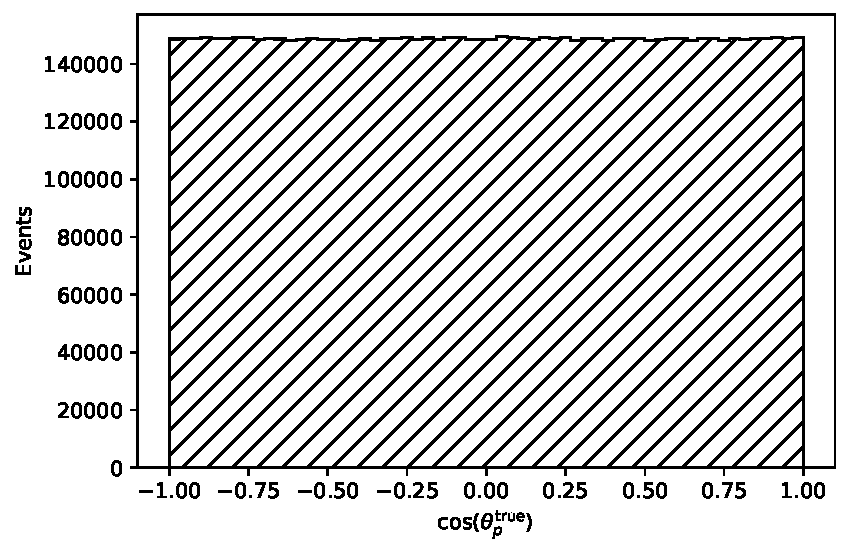
\includegraphics[height=.2\textheight]{graphics/05-angular_distributions/MCTRUTH_theta_true.pdf}
		\caption{}
		\label{fig:5:MCTRUTH_theta_true}
	\end{subfigure}
	\begin{subfigure}{.45\textwidth}
		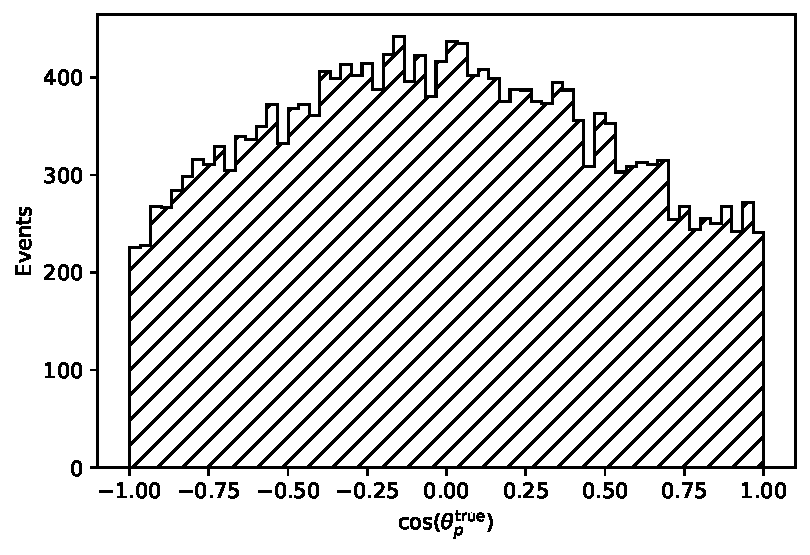
\includegraphics[height=.2\textheight]{graphics/05-angular_distributions/MCRECO_theta_true.pdf}
		\caption{}
		\label{fig:5:MCRECO_theta_true}
	\end{subfigure}
	\caption{Distributions of true values of \cthetap, as defined in \eqref{eq:5:helicity_theta}, for simulated \demonstratorshort events after all selection steps: \textit{(a)} using all generated events; \textit{(b)} using only reconstructed events.}
	\label{fig:5:theta_distributions_true}
\end{figure}

\begin{figure}[t]
	\centering
	\begin{subfigure}{.45\textwidth}
		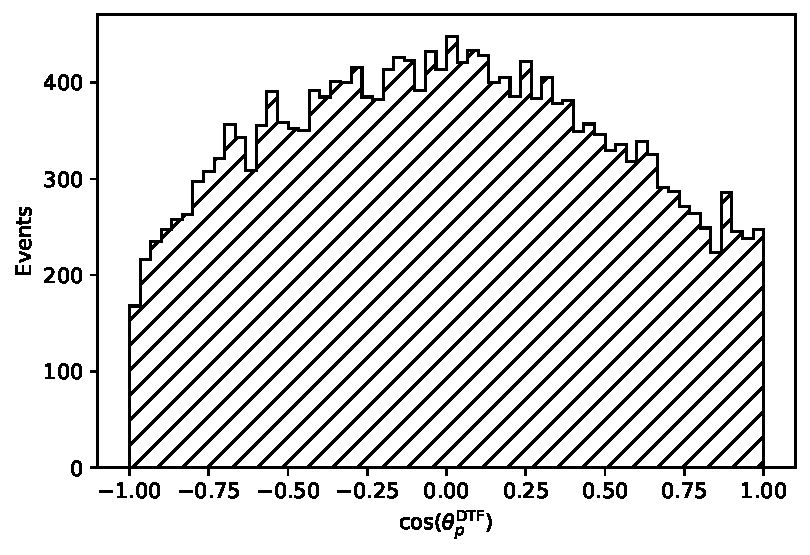
\includegraphics[height=.2\textheight]{graphics/05-angular_distributions/MCRECO_theta_reco.pdf}
		\caption{}
		\label{fig:5:MCRECO_theta_reco}
	\end{subfigure}
	\begin{subfigure}{.45\textwidth}
		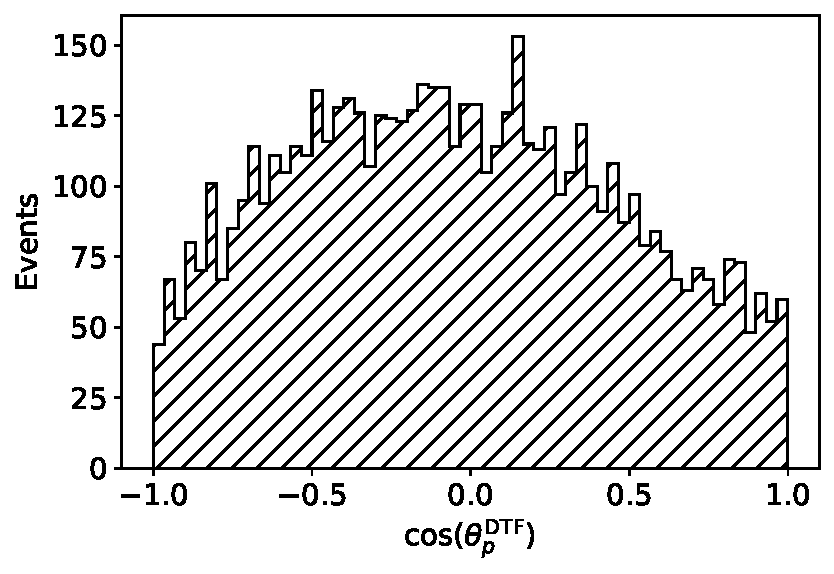
\includegraphics[height=.2\textheight]{graphics/05-angular_distributions/RUN2_theta_reco.pdf}
		\caption{}
		\label{fig:5:RUN2_theta_reco}
	\end{subfigure}
	\caption{Distributions of reconstructed $\cos\theta_p$, as defined in \eqref{eq:5:helicity_theta}, for simulated \demonstratorshort events \textit{(a)} and Run 2 data \textit{(b)} after all selection steps. Angle \thetap is computed using Decay Tree Fitter momenta with \jpsi and \lz mass constraints.}
	\label{fig:5:theta_distributions_reco}
\end{figure}

Figure \ref{fig:5:MCTRUTH_theta_true} depicts the \cthetap distribution of all (including non-reconstructed) simulated \demonstratorshort events using true $p$ and \pim momenta;
these events are generated without accounting for \lz polarization, hence the expected flatness of the distribution.
Figure \ref{fig:5:MCRECO_theta_true} shows true \cthetap distribution as well, this time only considering reconstructed events passing all selection steps. The comparison between these two figures highlights the angular acceptance effects that factor in the prospective \lz EDM/MDM measurement.

Affinity of Figure \ref{fig:5:MCRECO_theta_true} with Figure \ref{fig:5:MCRECO_theta_reco}, which shows reconstructed \cthetap using DTF momenta with \jpsi and \lz mass constraints, foreshadows the great angular resolution I will delve into in Section \ref{sec:5:angular_resolution}.
Finally, \cthetap in Run 2 data after all selection steps is shown in Figure \ref{fig:5:RUN2_theta_reco}:
this distribution is the overlap of contributions from \demonstratorshort signal with polarized \lz and from combinatorial background in the $\mu \pm 3\sigma$ signal region.

%\begin{figure}[t]
%	\centering
%	\begin{subfigure}{.45\textwidth}
%		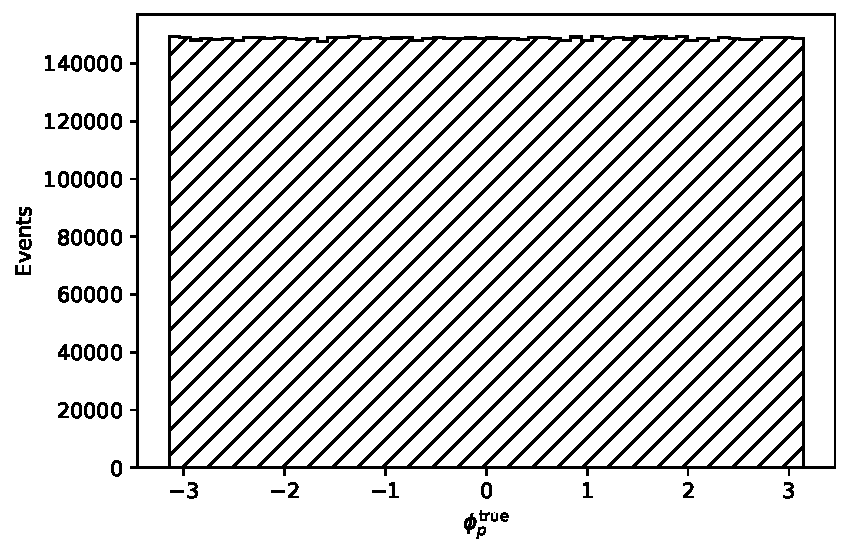
\includegraphics[height=.2\textheight]{graphics/05-angular_distributions/MCTRUTH_phi_true.pdf}
%		\caption{}
%		\label{fig:5:MCTRUTH_phi_true}
%	\end{subfigure}
%	\begin{subfigure}{.45\textwidth}
%		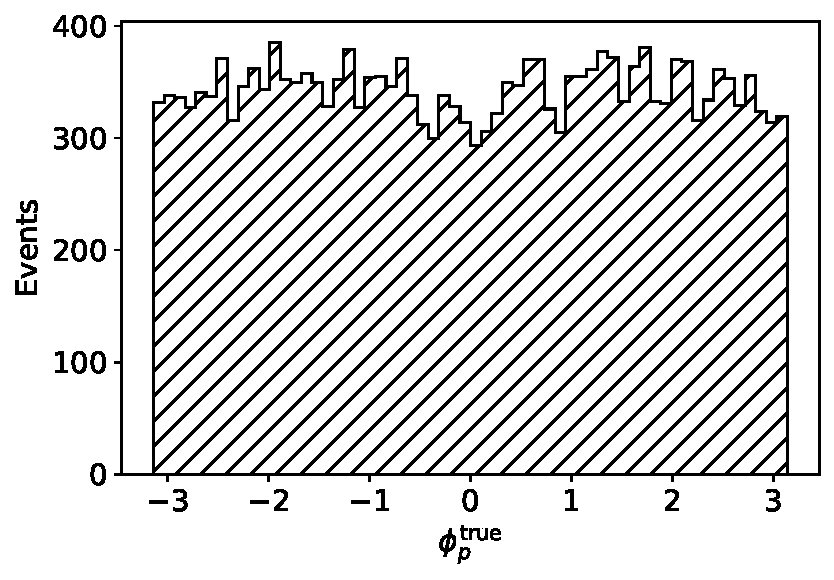
\includegraphics[height=.2\textheight]{graphics/05-angular_distributions/MCRECO_phi_true.pdf}
%		\caption{}
%		\label{fig:5:MCRECO_phi_true}
%	\end{subfigure}
%	\vskip .5\baselineskip
%	\begin{subfigure}{.45\textwidth}
%		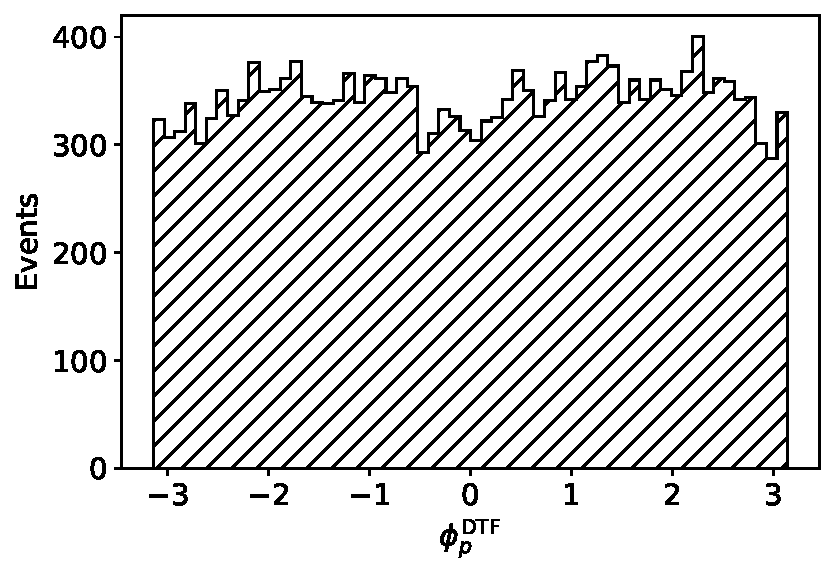
\includegraphics[height=.2\textheight]{graphics/05-angular_distributions/MCRECO_phi_reco.pdf}
%		\caption{}
%		\label{fig:5:MCRECO_phi_reco}
%	\end{subfigure}
%	\caption{Distributions of $\phi_p$, as defined in equation \eqref{eq:5:helicity_phi}, for simulated \demonstratorshort events after all selection steps: \textit{(a)} using all generated events and true momenta; \textit{(b)} using only reconstructed events and true momenta; \textit{(c)} using only reconstructed events and Decay Tree Fitter momenta with \jpsi and \lz mass constraints.}
%	\label{fig:5:phi_distributions}
%\end{figure}

\begin{figure}[t]
	\centering
	\begin{subfigure}{.45\textwidth}
		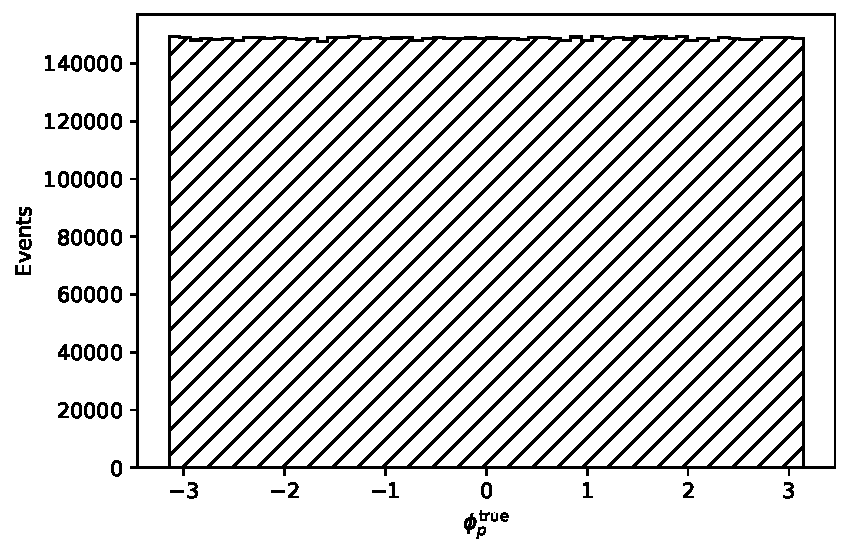
\includegraphics[height=.2\textheight]{graphics/05-angular_distributions/MCTRUTH_phi_true.pdf}
		\caption{}
		\label{fig:5:MCTRUTH_phi_true}
	\end{subfigure}
	\begin{subfigure}{.45\textwidth}
		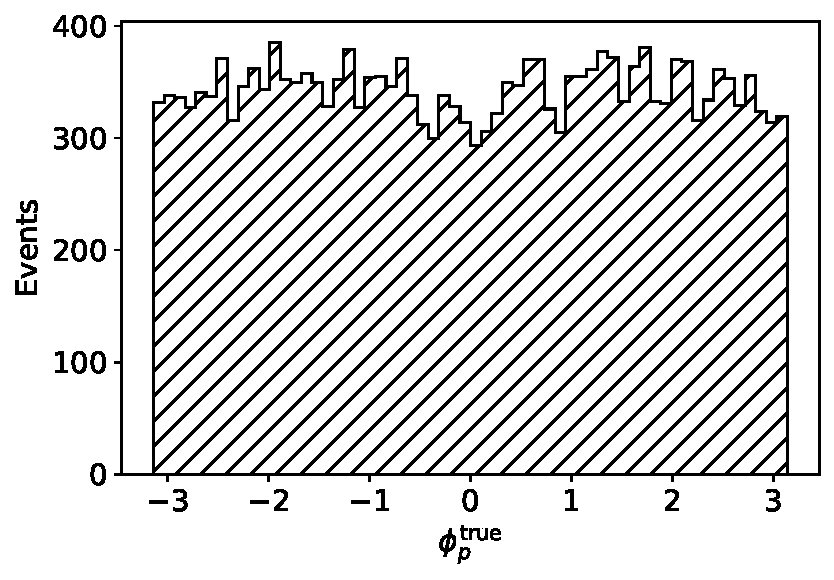
\includegraphics[height=.2\textheight]{graphics/05-angular_distributions/MCRECO_phi_true.pdf}
		\caption{}
		\label{fig:5:MCRECO_phi_true}
	\end{subfigure}
	\caption{Distributions of true values of \phip, as defined in \eqref{eq:5:helicity_phi}, for simulated \demonstratorshort events after all selection steps: \textit{(a)} using all generated events; \textit{(b)} using only reconstructed events.}
	\label{fig:5:phi_distributions_true}
\end{figure}

\begin{figure}[t]
	\centering
	\begin{subfigure}{.45\textwidth}
		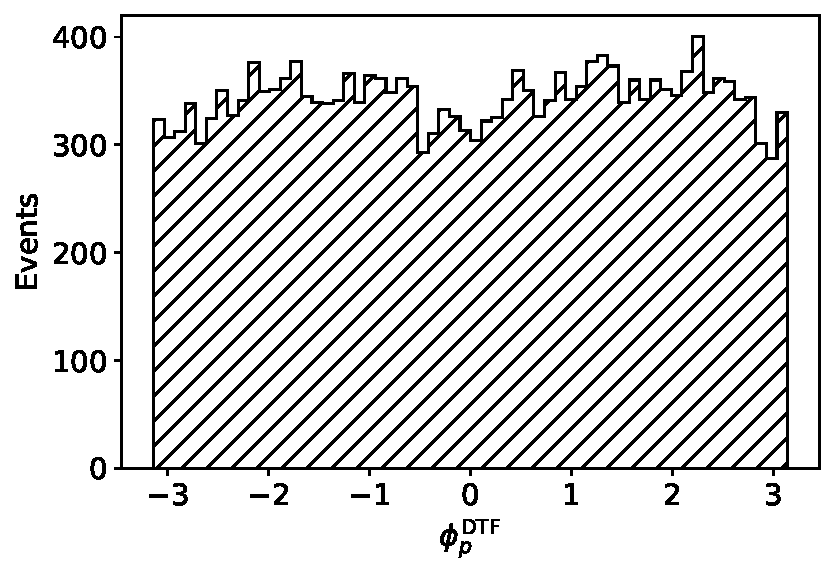
\includegraphics[height=.2\textheight]{graphics/05-angular_distributions/MCRECO_phi_reco.pdf}
		\caption{}
		\label{fig:5:MCRECO_phi_reco}
	\end{subfigure}
	\begin{subfigure}{.45\textwidth}
		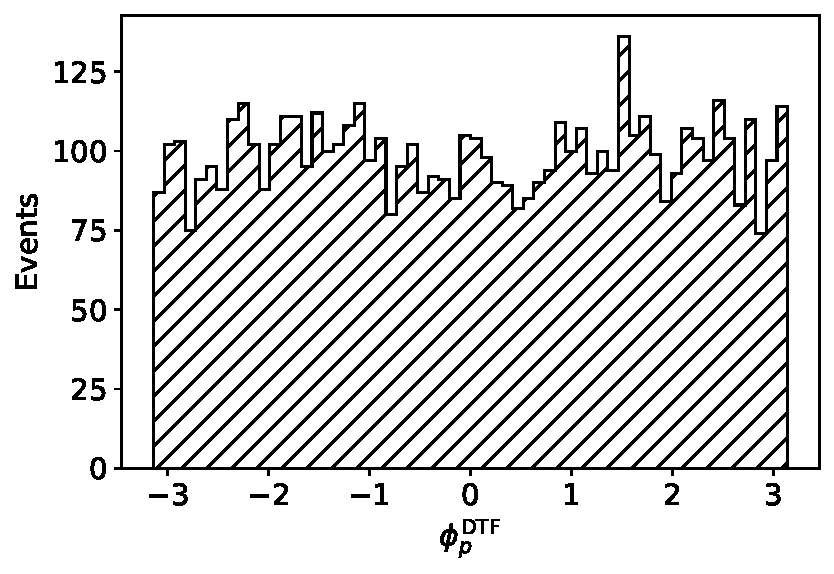
\includegraphics[height=.2\textheight]{graphics/05-angular_distributions/RUN2_phi_reco.pdf}
		\caption{}
		\label{fig:5:RUN2_phi_reco}
	\end{subfigure}
	\caption{Distributions of reconstructed \phip, as defined in \eqref{eq:5:helicity_phi}, for simulated \demonstratorshort events \textit{(a)} and Run 2 data \textit{(b)} after all selection steps. Angle \phip is computed using Decay Tree Fitter momenta with \jpsi and \lz mass constraints.}
	\label{fig:5:phi_distributions_reco}
\end{figure}

The same considerations made for \cthetap are valid for \phip distributions, which are reported in Figures \ref{fig:5:phi_distributions_true} and \ref{fig:5:phi_distributions_reco}.

\section{Proton angular resolution}
\label{sec:5:angular_resolution}

To assess the resolution on the proton angular distribution in reconstructed \demonstratorshort events, I defined 8 bins in $\cos\theta_p^\text{true}$ and 12 bins in $\phi_p^\text{true}$ and evaluated reconstructed angle dispersion in each truth bin. 
Angular resolution within a bin is defined as the root mean square error (RMSE) between reconstructed and true angles:
\begin{equation}
	\text{RMSE}(\psi) = \sqrt{\frac{1}{N} \sum_{i=1}^N {\left(\psi_i^\text{DTF} - \psi_i^\text{true}\right)}^2},
\end{equation}
with $\psi = \{\cos\theta_p, \phi_p$\}.

\begin{figure}[t]
	\centering
	\begin{subfigure}{.45\textwidth}
		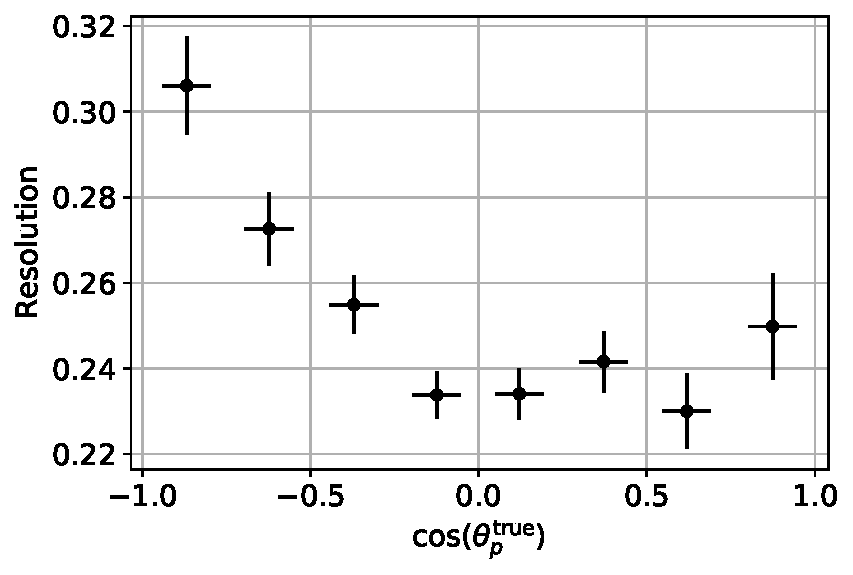
\includegraphics[height=.2\textheight]{graphics/05-angular_distributions/MCRECO_p_theta_resolution.pdf}
		\caption{}
		\label{fig:5:MCRECO_p_theta_resolution}
	\end{subfigure}
	\begin{subfigure}{.45\textwidth}
		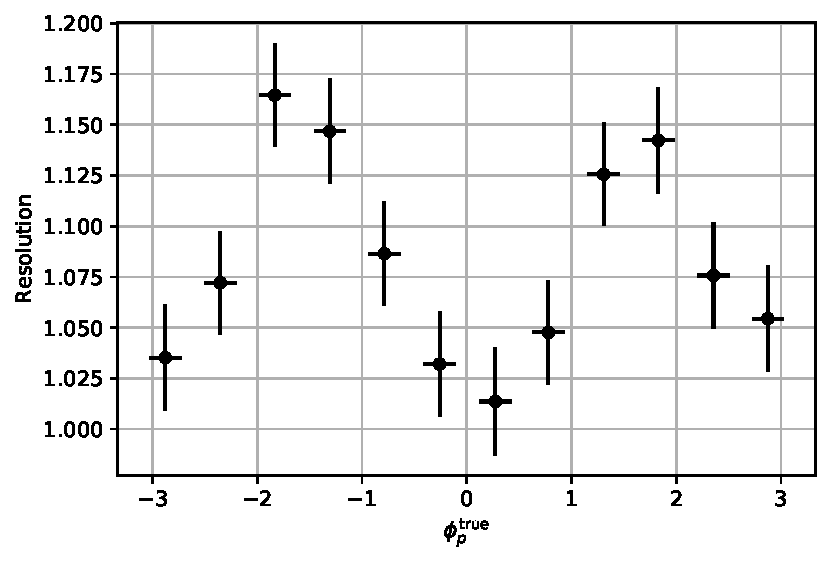
\includegraphics[height=.2\textheight]{graphics/05-angular_distributions/MCRECO_p_phi_resolution.pdf}
		\caption{}
		\label{fig:5:MCRECO_p_phi_resolution}
	\end{subfigure}
	\caption{Resolutions on $\cos\theta_p$ \textit{(a)} and $\phi_p$ \textit{(b)} as a function of the respective true values, computed on simulated \demonstratorshort events after all selection steps. Standard deviations within each bin are used as error bars on the $x$ axes.}
	\label{fig:5:angular_resolutions}
\end{figure}

Figure \ref{fig:5:MCRECO_p_theta_resolution} shows \cthetap resolution as a function of $\cos\theta_p^\text{true}$, demonstrating overall good resolution (in line with \cthetap variability within each bin).
The asymmetry in resolution at the opposite ends of the \cthetap spectrum, with a marked degradation of resolution around $\cos\theta_p^\text{true} \approx -1$, does not have a clear explanation;
however, as will be seen in Section \ref{sec:5:resolution_after_ghost}, this behaviour becomes noticeably less pronounced when the high-bias ghost vertex class of events is removed from the sample.

Figure \ref{fig:5:MCRECO_p_phi_resolution} depicts the same plot for azimuthal helicity angle \phip.
The only change from the \cthetap computation is that \phip resolution needs to account for the fact that $\phi=-\pi$ and $\phi=\pi$ are physically the same angle.
This has non-intuitive ripercussions when computing the residuals between $\phi_p^\text{true}$ and $\phi_p^\text{reco}$.
For instance, the nominal difference between $\phi_p^\text{reco}=\pi - \varepsilon$ and $\phi_p^\text{true}=-\pi + \varepsilon$ is $2\pi - 2\varepsilon$, but from a physical point of view the reconstructed angle is only off by $2\varepsilon$:
\begin{equation}
\lvert
\phi_p^\text{reco} - \phi_p^\text{true}
\rvert
=
|
\left( \pi - \varepsilon \right)
-
\left(- \pi + \varepsilon \right)
|
=
|
\underbrace{\pi - \left( -\pi \right)}_{\substack{=\,0 \\ \text{same angles}}}
- 2\varepsilon
|
= 2\varepsilon
\end{equation}
Given $\phi_1, \phi_2 \in [-\pi, \pi]$, this problem is easily solved by computing 
\begin{equation}
d \coloneqq \lvert \phi_1 - \phi_2 \rvert \bmod 2\pi
\end{equation}
and choosing as distance the lesser value between $d$ and $2\pi-d$.
%Given $\phi_1, \phi_2 \in [-\pi, \pi]$ and $\phi_1 \geq \phi_2$, this problem is solved by computing two distances
%\begin{subequations}
%\begin{align}
%	d_0 &= \lvert \phi_1 - \phi_2 \rvert \bmod 2\pi, \\
%	d_\pi &= \left(\lvert \pi - \phi_1 \rvert + \lvert \phi_2 + \pi \rvert \right) \bmod 2\pi,
%\end{align}
%\end{subequations}
%one passing through zero and the other through $\pm \pi$, and choosing the lesser one between the two.


The range of variability for \phip resolution is even smaller compared to \cthetap, which is consistent with the expected azimuthal symmetry of the LHCb detector;
nevertheless, resolution gets noticeably worse for $\phi_p \approx \pm \frac{\pi}{2}$.
The shape of Figure \ref{fig:5:MCRECO_p_phi_resolution} shows remarkable correlation with the observed angular \phip acceptance in reconstructed events (see Figure \ref{fig:5:MCRECO_phi_reco}), suggesting that the two effects might share a common source;
moreso than in the \cthetap case, this effect is all but removed when excluding ghost vertex events.

\begin{figure}[t]
	\centering
	\begin{subfigure}{.45\textwidth}
		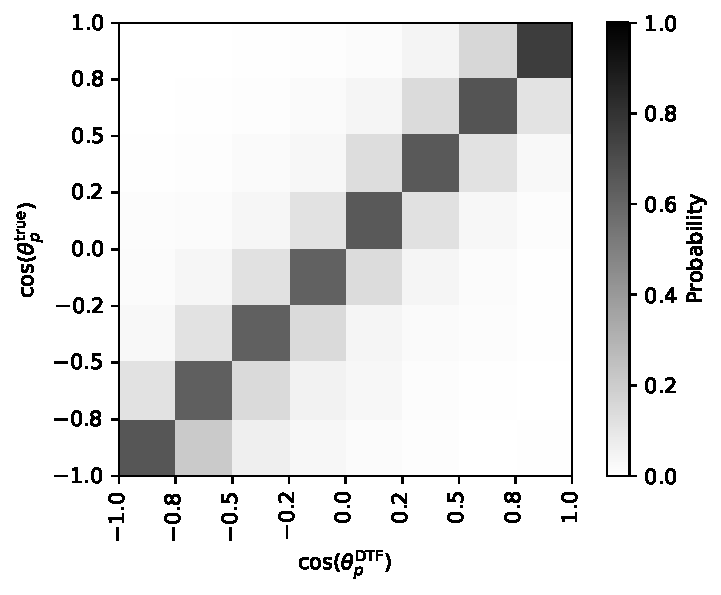
\includegraphics[width=\textwidth]{graphics/05-angular_distributions/MCRECO_p_theta_migration.pdf}
		\caption{}
		\label{fig:5:MCRECO_p_theta_migration}
	\end{subfigure}
	\begin{subfigure}{.45\textwidth}
		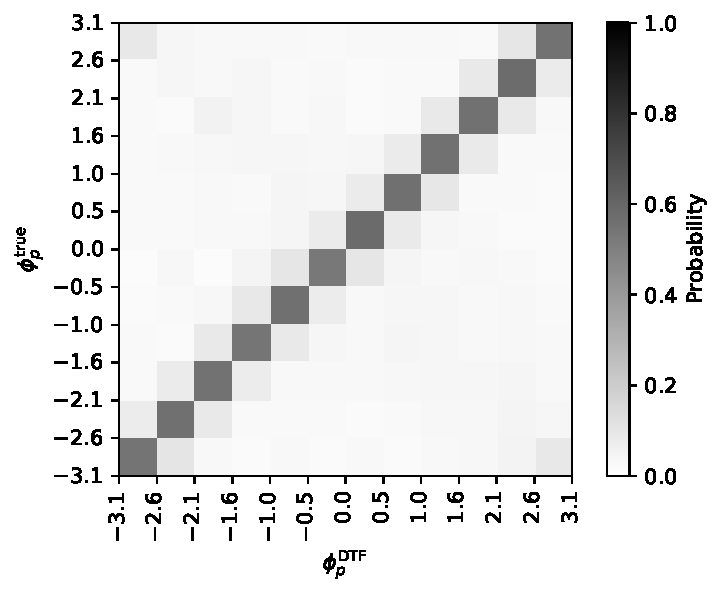
\includegraphics[width=\textwidth]{graphics/05-angular_distributions/MCRECO_p_phi_migration.pdf}
		\caption{}
		\label{fig:5:MCRECO_p_phi_migration}
	\end{subfigure}
	\caption{Migration matrices of $\cos\theta_p$ \textit{(a)} and $\phi_p$ \textit{(b)}, computed on simulated \demonstratorshort events after all selection steps. Probabilities and chromatic scale are normalized on true bins.}
	\label{fig:5:angular_migration_matrices}
\end{figure}

The general soundness of proton angular reconstruction translates in the \cthetap and \phip migration matrices presented in Figure \ref{fig:5:angular_migration_matrices}:
each $(i,j)$ bin is color-coded according to the probability $P(i \rightarrow j)$ of migration from $\psi_i$ in true bin $i$ to $\psi_j$ in reconstructed bin $j$. Probabilities are normalized to unity in the true bin, that is
\begin{equation}
	\sum_{j \in \{ \text{reco bins} \}} P(i\rightarrow j) = 1.
\end{equation}
The matrices are both diagonal net of dispersion effects, demonstrating the lack of meaningful bias in reconstruction of \cthetap and \phip.
In Figure \ref{fig:5:MCRECO_p_phi_migration}, the top left and bottom right bins are evidence of the looping effect of the $[-\pi,\pi]$ range of values for \phip, both harboring events from the physically adjacent bottom left and top right bins.

\subsection{Impact of ghost vertex events}
\label{sec:5:resolution_after_ghost}

\begin{figure}[t]
	\centering
	\begin{subfigure}{.45\textwidth}
		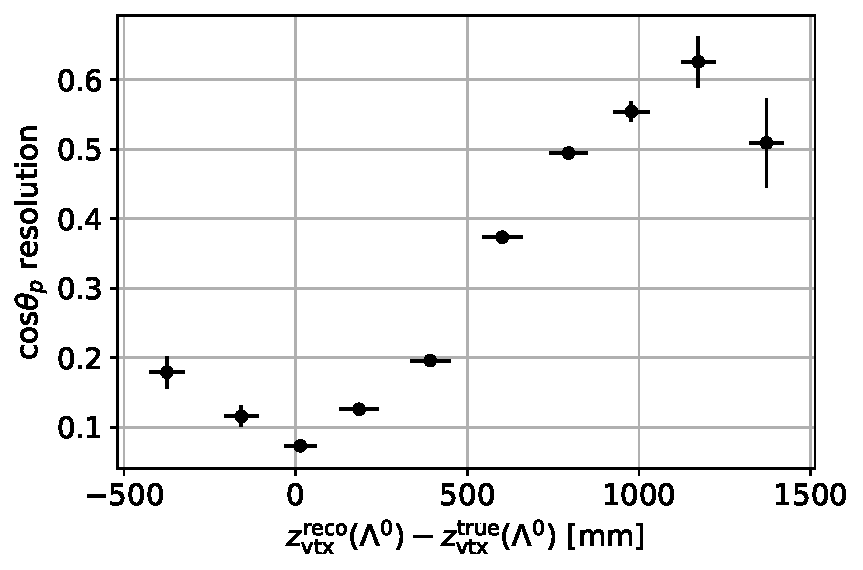
\includegraphics[width=\textwidth]{graphics/05-angular_distributions/MCRECO_p_theta_resolution_vs_L_endvertex_z_bias.pdf}
		\caption{}
		\label{fig:5:theta_resolution_vs_vertex_bias}
	\end{subfigure}
	\begin{subfigure}{.45\textwidth}
		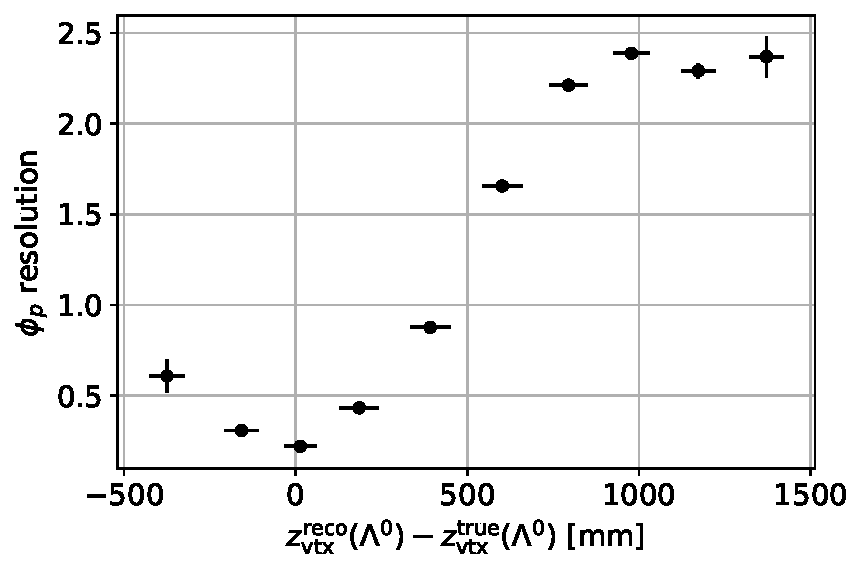
\includegraphics[width=\textwidth]{graphics/05-angular_distributions/MCRECO_p_phi_resolution_vs_L_endvertex_z_bias.pdf}
		\caption{}
		\label{fig:5:phi_resolution_vs_vertex_bias}
	\end{subfigure}
	\caption{Angular resolutions on $\cos\theta_p$ \textit{(a)} and $\phi_p$ \textit{(b)} as a function of bias on reconstructed $z_\text{vtx}^\Lambda$, computed on simulated \demonstratorshort events after all selection steps.}
	\label{fig:5:angular_resolution_vs_vertex_bias}
\end{figure}

As discussed in Section \ref{sec:lambda_endvertex_bias}, resolution in the $z_\text{vtx}^\Lambda$ component of the \lambdadecay decay vertex is affected by a significant $\approx \SI{14}{\centi\meter}$ positive bias, whose distribution is depicted in Figure \ref{fig:3:lz_endvertex_bias_linear}.
The detrimental effect of this bias is seen in Figure \ref{fig:5:angular_resolution_vs_vertex_bias}, showing proton \cthetap and \phip resolutions as a function of $z_\text{vtx}^\Lambda$ bias:
resolutions worsen by a factor of five or more when going from $z_\text{vtx}^\text{reco} - z_\text{vtx}^\text{true} \approx \SI{0}{\meter}$ to $\SI{1.2}{\meter}$.
This is to be expected since poor \lz vertex reconstruction affects resolution on proton momenta.

%Resolutions reported in Figure \ref{fig:5:angular_resolutions} are computed on a simulated sample with subpar resolution on the \lz decay vertex, as seen from Figure \ref{fig:3:lz_endvertex_bias_linear}.
%Roughly $\approx 26\%$ of the data pass the $\Delta h > 1$ criterium, which I have shown to be a good indicator of the fraction of ghost vertex events.

Studies detailed in Section \ref{sec:3:ghost_vertex} illustrate that most highly biased events can be traced back to the <<ghost vertex>> problem, whereby the bending of $p\pi^-$ tracks in the $xz$ plane due to the LHCb magnetic field creates a second crossing point which provides a local $\chi^2$ minimum for the Vertex Fitter algorithm to converge at.
This issue affects almost one third of \demonstratorshort simulated events and is only found in T tracks, since other track types come from particles produced upstream of the magnet.
%Only arising when working with T tracks, as other track types come from particles produced upstream of the magnet, this problem is under-researched due to the historical rare employment of T tracks in physics analyses at LHCb.

\begin{figure}[t]
	\centering
	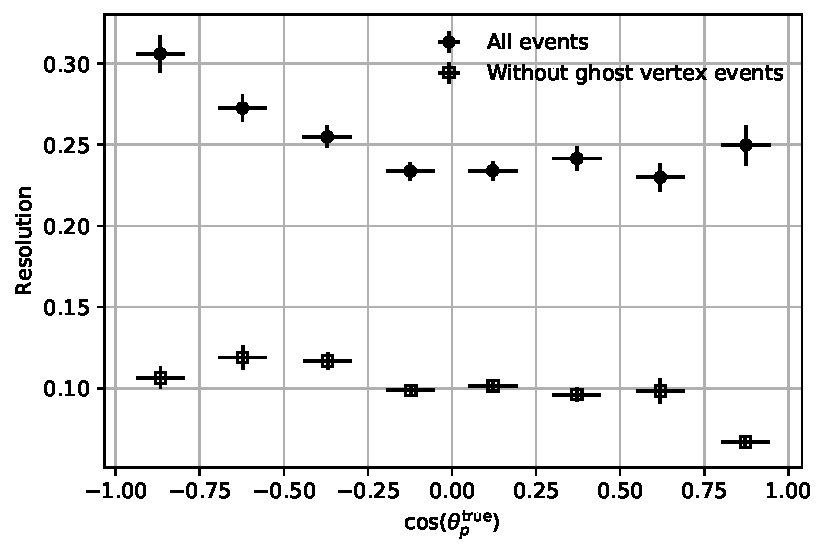
\includegraphics[width=.7\textwidth]{graphics/05-angular_distributions/MCRECO_p_theta_resolution_nocross.pdf}
	\caption{Angular resolution on \cthetap as a function of its true values. Resolution is computed on simulated \demonstratorshort events after all selection steps, including (\textit{filled circles}), removing (\textit{empty squares}), and only keeping (\textit{filled triangles}) \lambdadecay ghost vertex events.}
	\label{fig:5:theta_resolution_nocross}
\end{figure}

\begin{figure}[t]
	\centering
	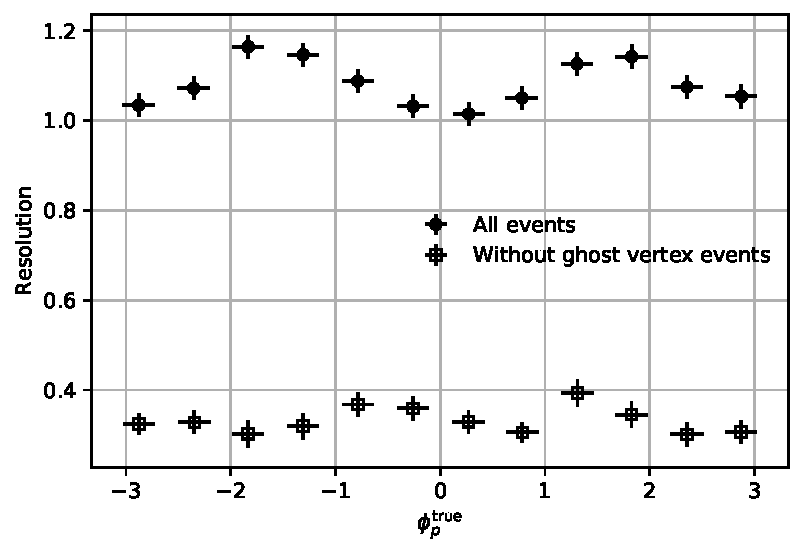
\includegraphics[width=.7\textwidth]{graphics/05-angular_distributions/MCRECO_p_phi_resolution_nocross.pdf}
	\caption{Angular resolution on \phip \textit{(a)} as a function of true values. Resolution is computed on simulated \demonstratorshort events after all selection steps, including (\textit{filled circles}), removing (\textit{empty squares}), and only keeping (\textit{filled triangles}) \lambdadecay ghost vertex events.}
	\label{fig:5:phi_resolution_nocross}
\end{figure}

Work is currently underway in the Milan and Valencia LHCb research groups to solve or mitigate the ghost vertex issue, with the goal of standardizing \lz vertex resolution to the non-ghost-vertex baseline of $\approx \SI{5.2}{\centi\meter}$.
Should such an endeavour be successful, Figure \ref{fig:5:angular_resolution_vs_vertex_bias} proves it would have a significant effect on the proton angular resolution and thus on the prospective measurement of \lz electromagnetic dipole moments.
As a proof of concept study, I computed angular resolutions for \cthetap and \phip excluding ghost vertex events, the latter being defined with the locus of points from \eqref{eq:3:psih_banana}.
Results are shown in Figures \ref{fig:5:theta_resolution_nocross} and \ref{fig:5:phi_resolution_nocross}:
in both cases resolution improves by a factor 2--3 in all truth bins.
Furthermore, the deviation from flat resolutions seen in Figure \ref{fig:5:MCRECO_p_theta_resolution} and \ref{fig:5:MCRECO_p_phi_resolution} are significantly suppressed when removing ghost vertex events, identifying them as the primary culprits.
%A soft slope is still present in \cthetap resolution without ghost vertices:
%this can partially be attributed to the correlation between \cthetap and proton $p_z$, as protons with $\cos\theta_p < 0$ are produced with smaller $p_z$ and lower momentum negatively affects angular reconstruction.

\section{Resolution effects on expected proton angular distributions}
As seen in the previous section, resolution on proton \cthetap and \phip production angles can be significantly improved with the removal of ghost vertex events.
As a first test of the impact of this enhancement on the prospective measurement of \lz electromagnetic dipole moments, I  generated samples of $n={10}^6$ \demonstratorshort events under the following simplifying assumptions:
\begin{itemize}
	\item \lz are produced with $\vec{p} = p \hat{z}$, $\beta=1$ and maximal longitudinal polarization;
	\item all \lz traverse the full $D_y = \SI{4}{\tesla\meter}$ LHCb magnetic field before decaying;
	\item no experimental resolutions are considered outside of the ones on \cthetap and \phip;
	\item all acceptance effects are neglected;
	\item the \lz gyroelectric and gyromagnetic factors are $d=0$ and $g=1.226$ \cite{PDG} respectively.
\end{itemize}
Proton production angles were extracted with a standard Monte Carlo rejection sampling algorithm (commonly also known as \textit{accept-reject} algorithm) using angular distribution \eqref{eq:angular_distribution_cap1}.

\begin{figure}[t]
	\centering
	\begin{subfigure}{.45\textwidth}
		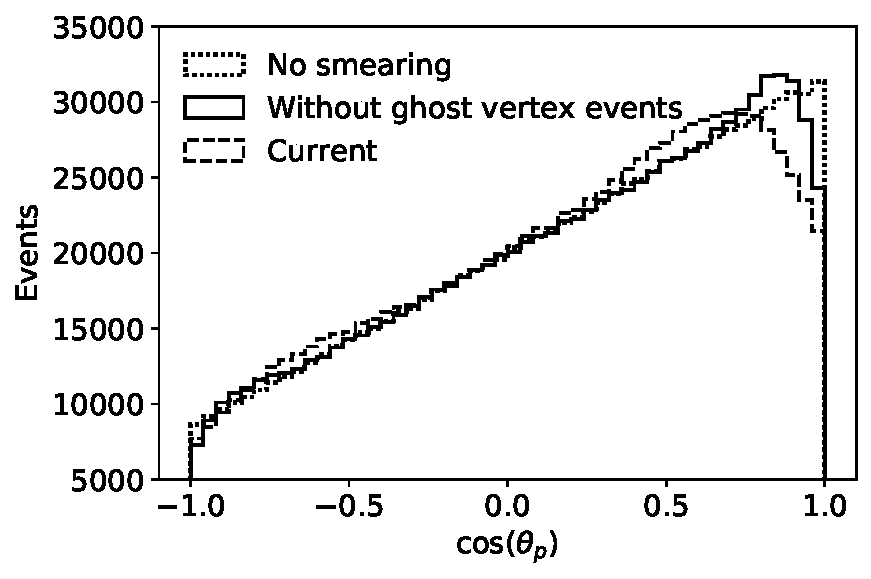
\includegraphics[width=\textwidth]{graphics/05-angular_distributions/ctheta_bw.pdf}
		\caption{}
		\label{fig:5:ctheta_bw}
	\end{subfigure}
	\begin{subfigure}{.45\textwidth}
		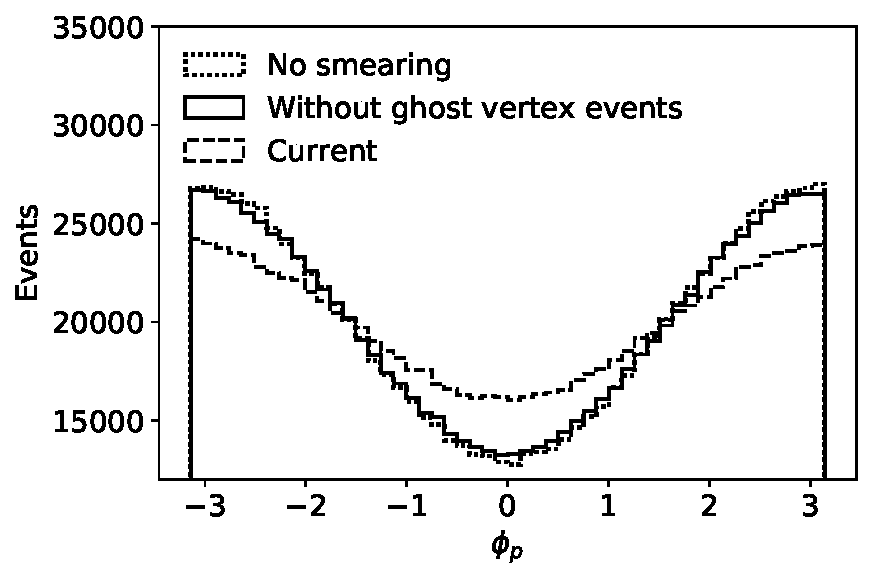
\includegraphics[width=\textwidth]{graphics/05-angular_distributions/phi_bw.pdf}
		\caption{}
		\label{fig:5:phi_bw}
	\end{subfigure}
	\caption{A.}
	\label{fig:5:ctheta_phi_bw}
\end{figure}

The effect of angular resolutions on the measurement of \cthetap and \phip was implemented with a per-event Gaussian smearing:
the generated angles are used as mean value $\mu$ of a Gaussian distribution $\mathcal{N}(\mu,\sigma^2)$, with $\sigma$ being the average desired resolution, and new \cthetap and \phip are chosen according to $\mathcal{N}$.
I produced three data samples: a <<perfect>> sample without any smearing, a sample matching resolution with the removal of ghost vertex events, and a sample matching the current resolution (i.e. with all reconstructed \demonstratorshort events).

\begin{figure}[t]
	\centering
	\begin{subfigure}{.45\textwidth}
		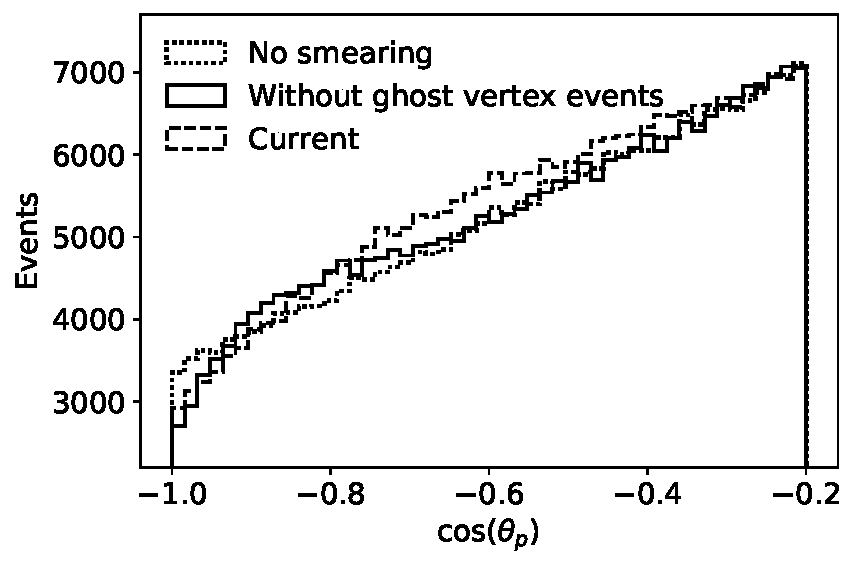
\includegraphics[width=\textwidth]{graphics/05-angular_distributions/ctheta_bw_left.pdf}
		\caption{}
		\label{fig:5:ctheta_bw_left}
	\end{subfigure}
	\begin{subfigure}{.45\textwidth}
		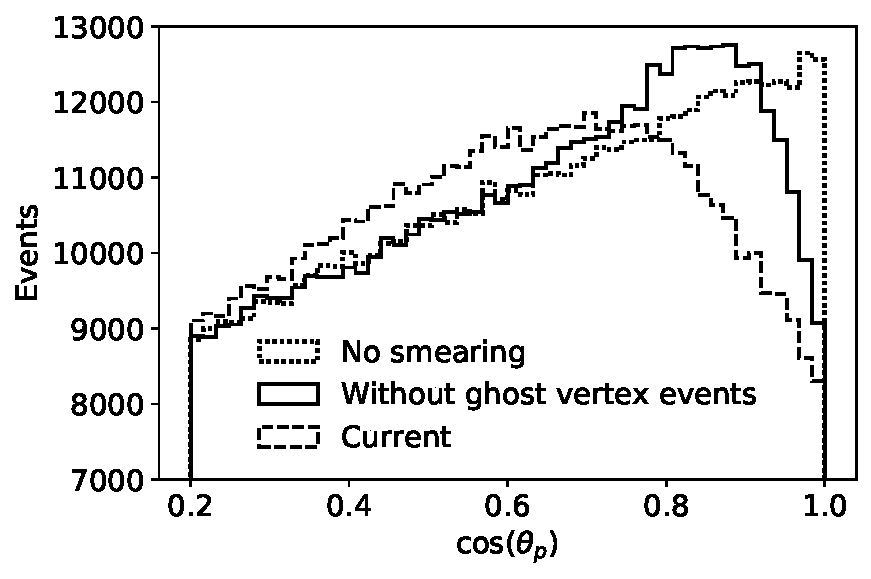
\includegraphics[width=\textwidth]{graphics/05-angular_distributions/ctheta_bw_right.pdf}
		\caption{}
		\label{fig:5:ctheta_bw_right}
	\end{subfigure}
	\caption{A.}
	\label{fig:5:ctheta_bw_details}
\end{figure}

\begin{figure}[t]
	\centering
	\begin{subfigure}{.45\textwidth}
		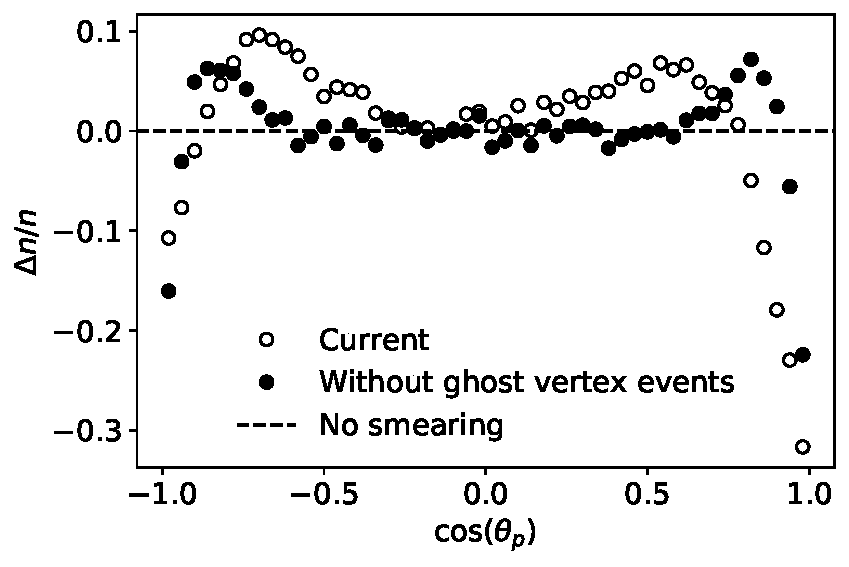
\includegraphics[width=\textwidth]{graphics/05-angular_distributions/ctheta_bw_residuals.pdf}
		\caption{}
		\label{fig:5:ctheta_bw_residuals}
	\end{subfigure}
	\begin{subfigure}{.45\textwidth}
		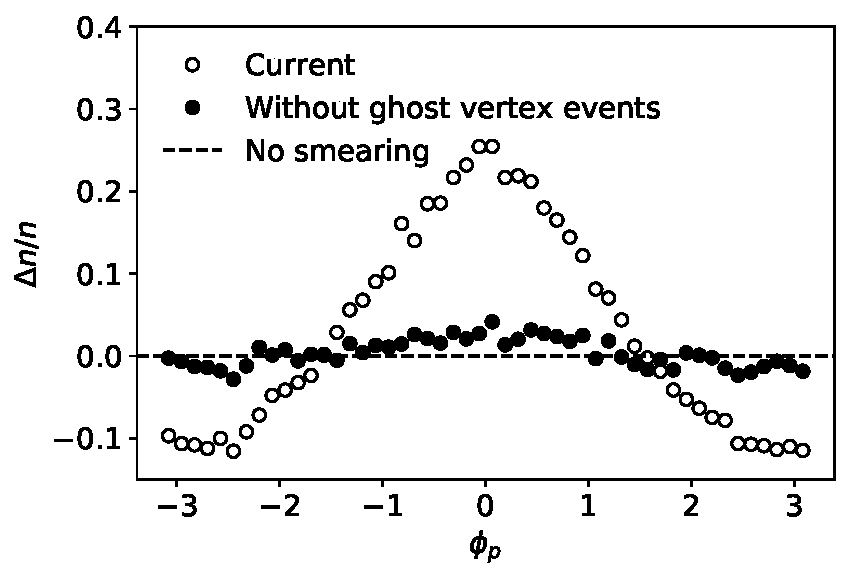
\includegraphics[width=\textwidth]{graphics/05-angular_distributions/phi_residuals.pdf}
		\caption{}
		\label{fig:5:phi_bw_residuals}
	\end{subfigure}
	\caption{A.}
	\label{fig:5:bw_residuals}
\end{figure}

